%not in details put in introduction

\section{Introduction}

The main goal of this research is to distinguish all dynamic objects present in the scene. The scene is observed from a camera installed in a car.

This setup brings one issue: \textit{apriori} all the objects are moving, since the car moves in the scene, thus the entire scene seems to change in every instant. 

When we talk about distinguish static and dynamic object, we are refeering them to be dynamic or static state with respect to the earth, not to the vehicle.

\section{Demonstrator configuration} %configuration of the lasers, diagram
\label{sec:demonstrator}

Our testbed used is a Toyota Lexus car equipped with two LIDAR lasers scanner (Section~\ref{sec:testbed} for the specification) installed in the frontal bumber (Figure~\ref{fig:demonstrator:birdeye}).

\begin{figure}[h]
   \centering
     \begin{tabular}{lr}
       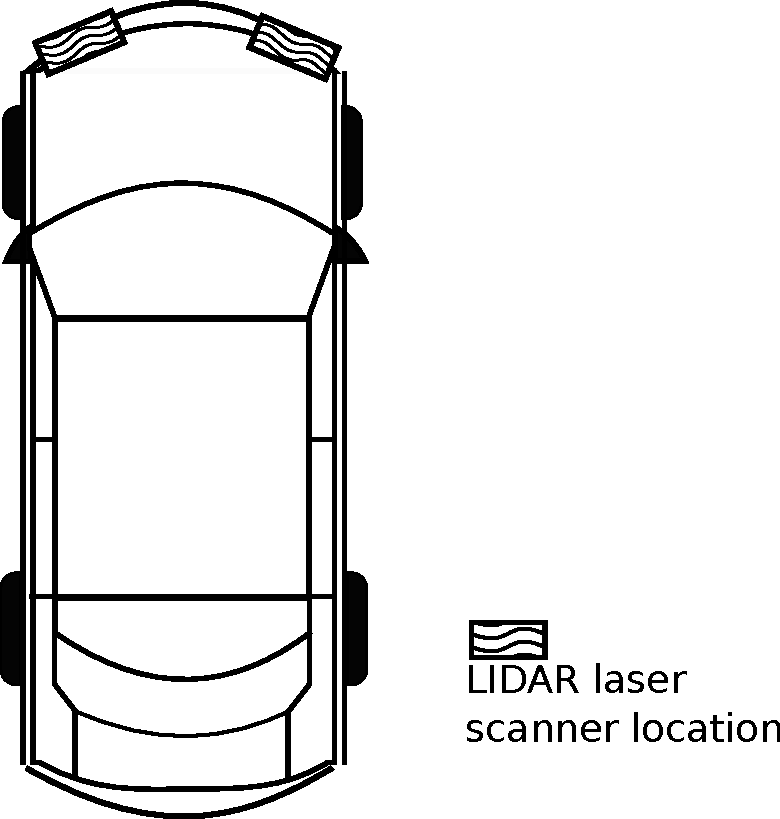
\includegraphics[scale=0.4]{img/fig:demonstrator:birdeye}
     \end{tabular}
   \caption{Bird-eye view: LIDAR laser scanners location}
   \label{fig:demonstrator:birdeye}
\end{figure}

The LIDAR is distributed in layers (Figure~\ref{fig:demonstrator:lateral}) and scanning range (Figure~\ref{fig:demonstrator:superior}). 

There are four layers in total, each layer disposed in different angles. The terrain is considered as base for the formation of this angle. This angle is constructed by the angle formed between an imaginary line, which is parallel to the road surface, and the layer. Those angles are depicted in the Figure~\ref{fig:demonstrator:lateral}.

\begin{figure}[h]
   \centering
     \begin{tabular}{lr}
       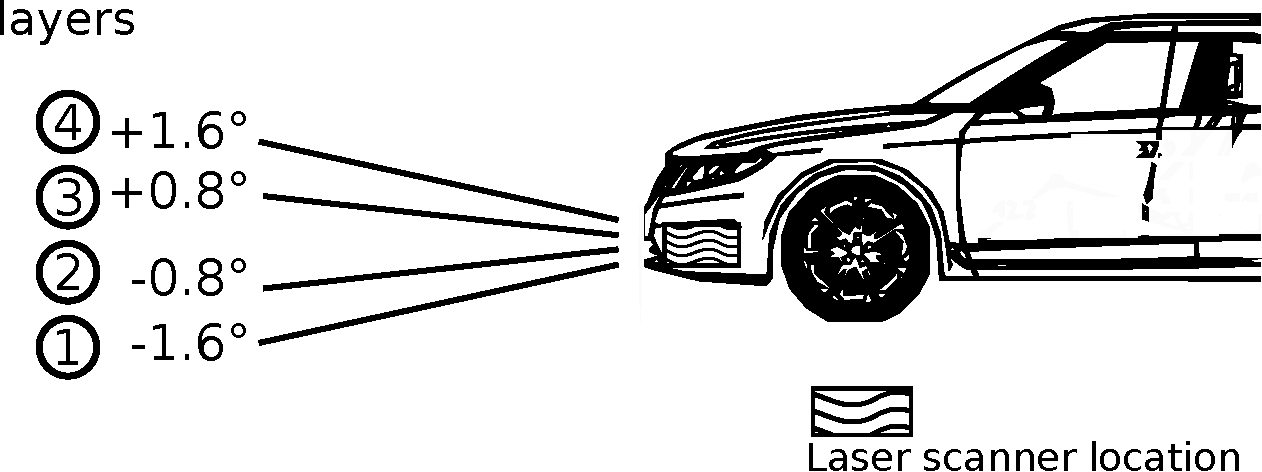
\includegraphics[scale=0.5]{img/fig:demonstrator:lateral}
     \end{tabular}
   \caption{Lateral view: Four layers of the left LIDAR laser scanner}
   \label{fig:demonstrator:lateral}
\end{figure}

Every layer spread in a given range, in the Table~\ref{tab:beam:interception} we can see the layers and their specific range. The LIDAR laser scanner used in our tests have the $+0.5^circ$ resolution. 

To calculate the number of beams available in the layer $\ell$, we apply the Equation~\ref{eq:totalbeams}, where the functions $min$ and $max$ are the minimum and maximum  , respectively, range available for the layer $\ell$, and the function $resolution$ gives the resolution of the LIDAR laser scanner $\rho$, this specification is given by the manufacturer. 

From that we can calculate the number of beams we have in the layer according with its range, let's take as example the first layer and calculate the number of beans available in this layer. The first layer has a range that varies from $+35^\circ$ to $-60^\circ$ (minimum and maximum range, respectively), the resolution is $+0.5^\circ$, according to the specification of the manufacturer, Equation~\ref{eq:totalbeams} this layer contains $190$ beams.

\begin{equation}
\label{eq:totalbeams}
beams_{total}(\ell)=\frac{|max(\ell)-min(\ell)|}{resolution(\rho)}
\end{equation}


From every invidual beam is possible to obtain the distance between the LIDAR laser scanner and the first object to intercept this beam of light.

\begin{figure}[h]
   \centering
     \begin{tabular}{lr}
       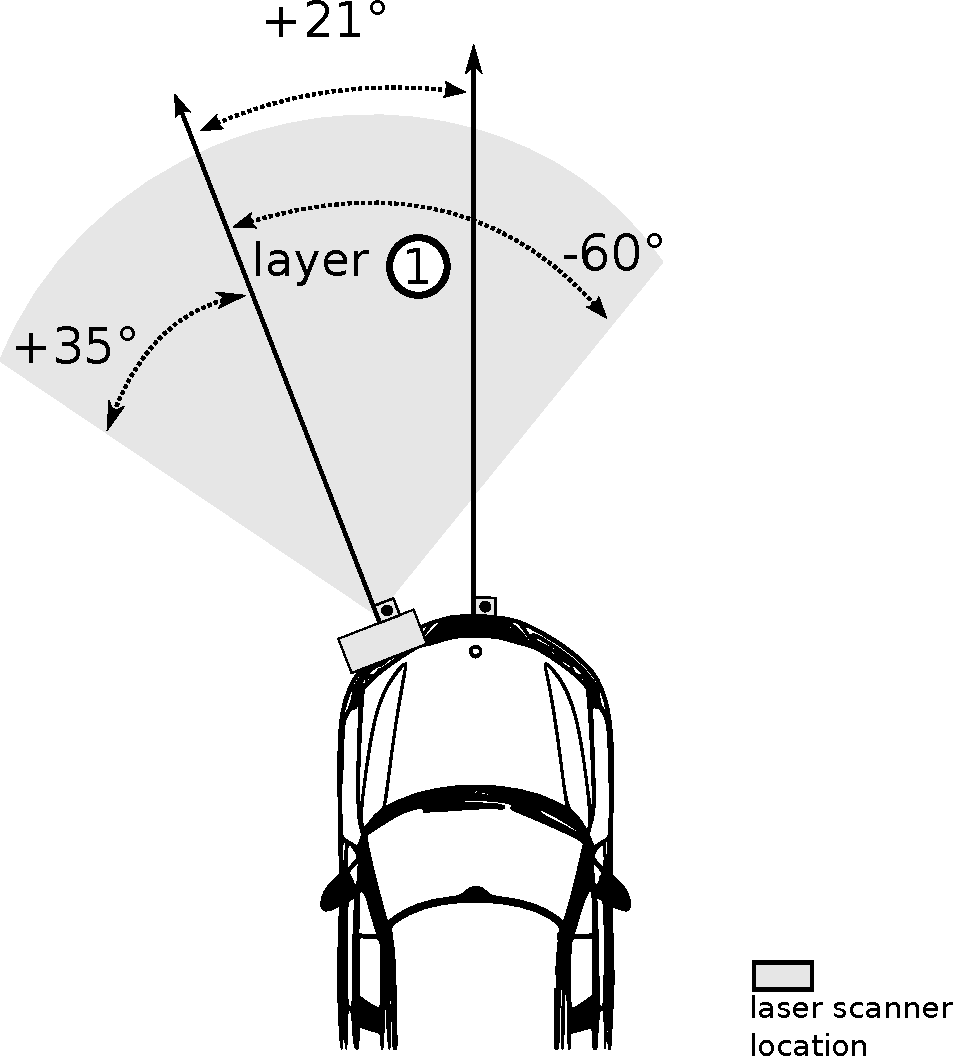
\includegraphics[scale=0.5]{img/fig:demonstrator:superior}
     \end{tabular}
   \caption{Bird-eye view: Left LIDAR laser scanner range, for the first layer}
   \label{fig:demonstrator:superior}
\end{figure}


\begin{table}
\label{tab:beam:interception}
	\begin{center}
	    \begin{tabular}{ | c | c | c | c | c |}
		    \hline
		    Layer & $+50^\circ$ & $+35^\circ$ & $-50^\circ$ & $-60^\circ$ \\ \hline
		    4 & + & + & + &  \\ \hline
		    3 & + & + & + &  \\ \hline
		    2 &  & + & + & + \\ \hline
		    1 &  & + & + & + \\ \hline
		    $\cap$ &  & + & + &  \\ \hline
	    \end{tabular}
	\end{center}
    \caption{Layers and the horizontal distribution of the beams}
\end{table}

Multiple sensor usage in the demonstrator makes of it a complex system, due to the number of data gathered and overlaped information. Thus, all sensor information must be carried in a consistent manner and this is done by fusing the sensor information, more details about how this is done in the Section~\ref{sec:sensor:fusion}.

\section{Sensor pre-processing} %fusion module
\label{sec:sensor:fusion}

% in the last subsection, output form (occupancy grid), digrams; explains that this is our input

\subsection{Purpose}

The demonstrator car is composed with two LIDAR laser scanner sensors, as we saw in the Section~\ref{sec:sensor:fusion}. Each of the LIDAR laser scanner is composed of few layers and each layer contains several beams. Those beams are spread horizontally in a given angle range, the ranging (initial and final angles) depends on the layer.

\begin{figure}[h]
   \centering
     \begin{tabular}{lr}
       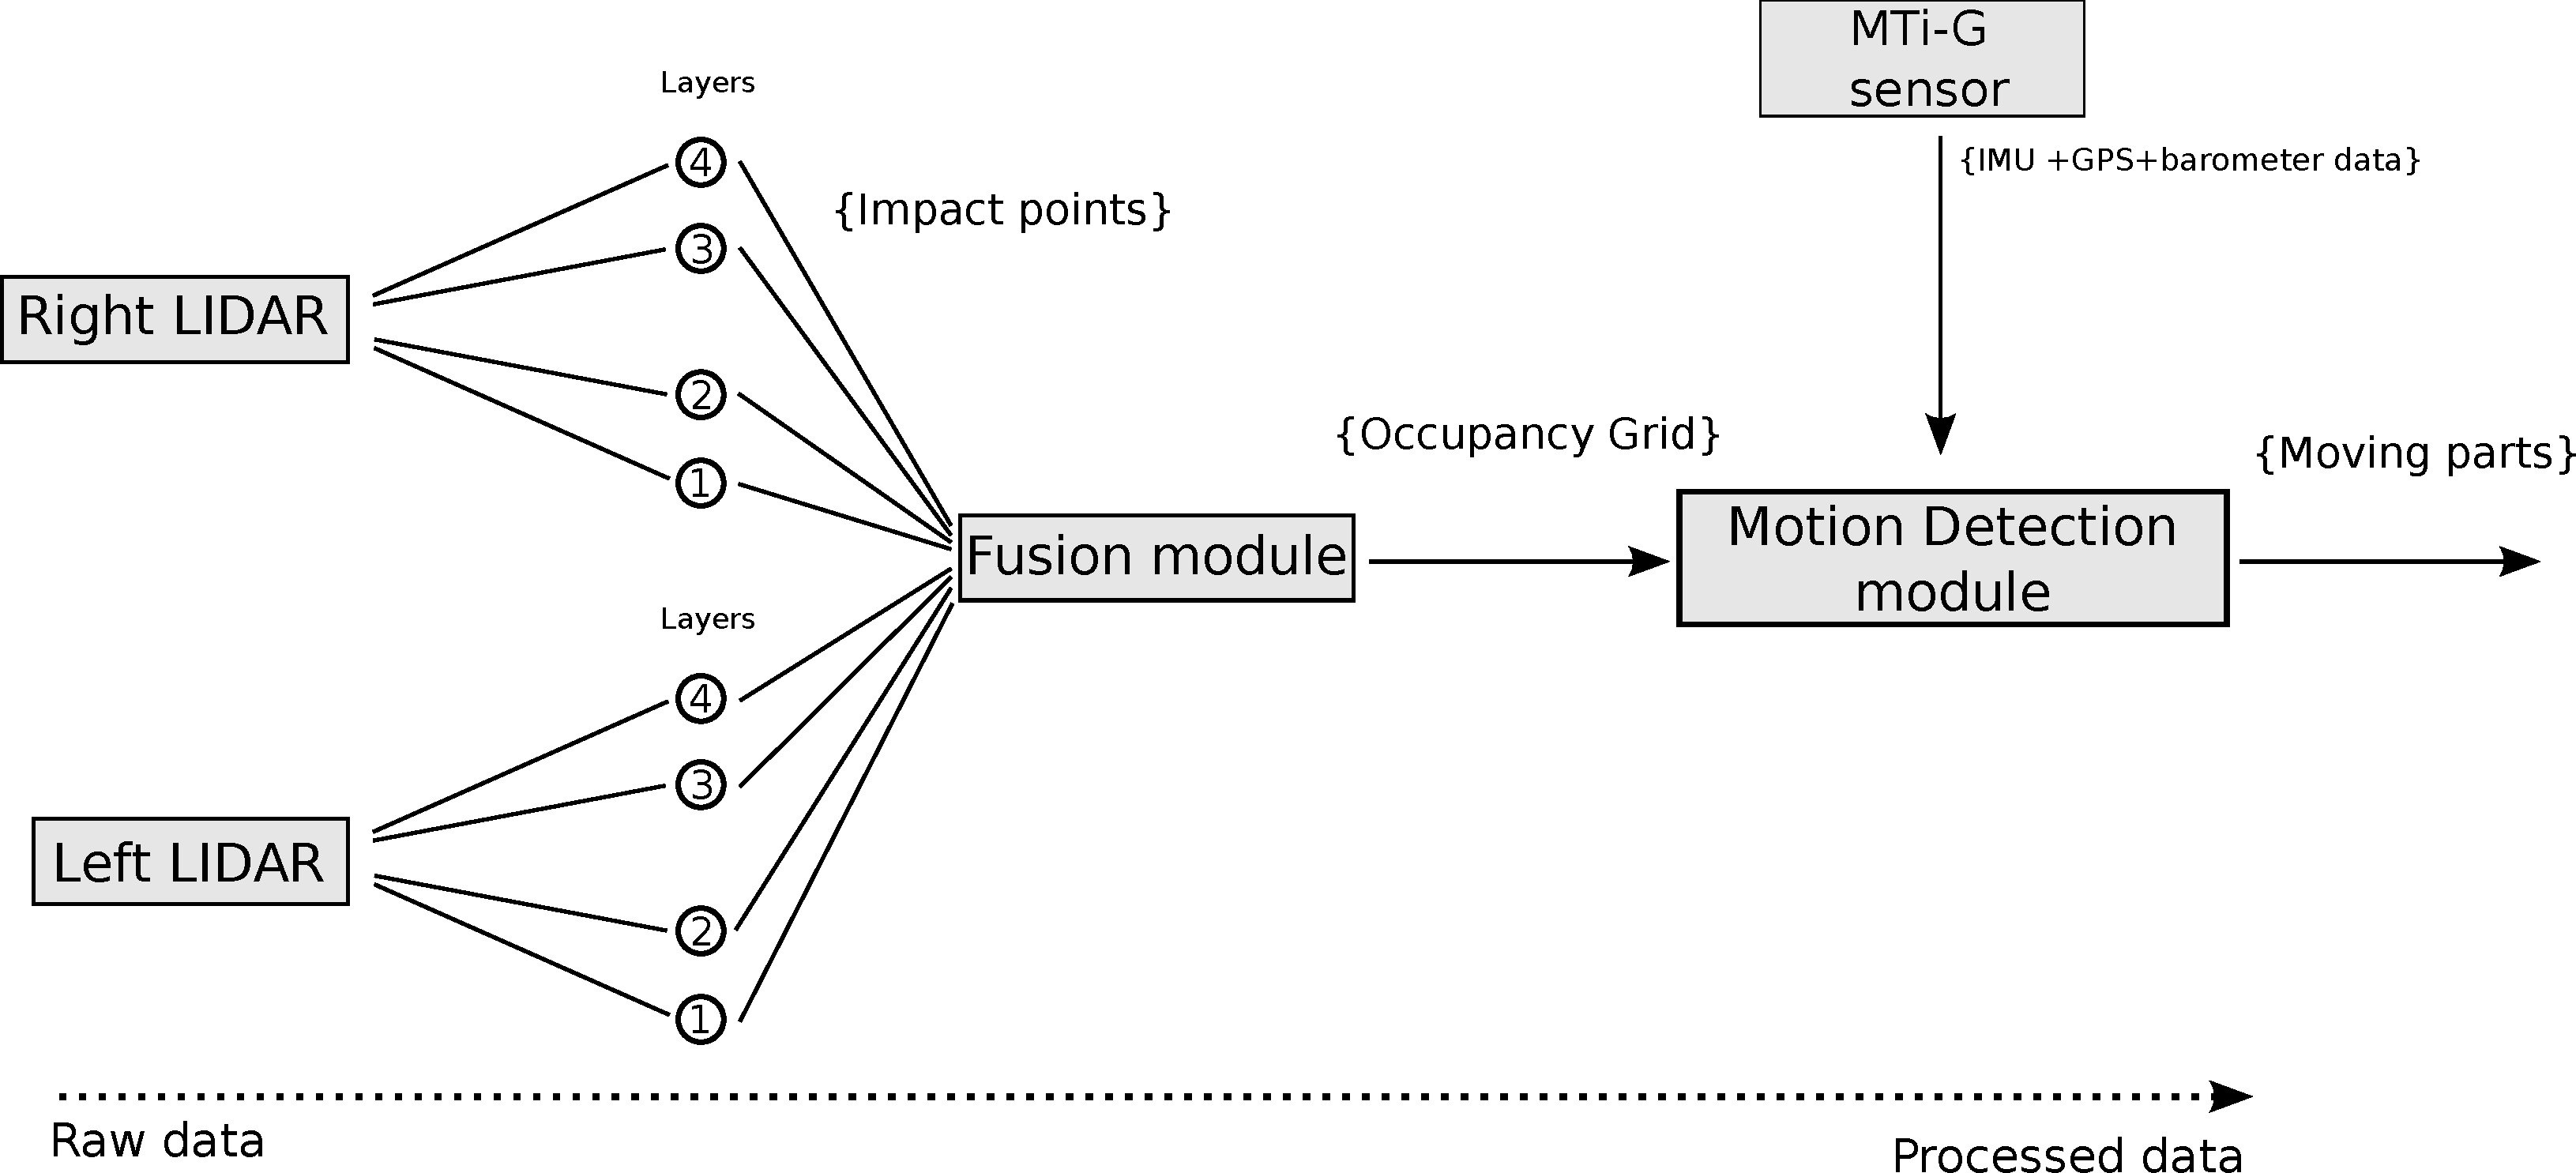
\includegraphics[scale=0.30]{img/fig:motion:framework}
     \end{tabular}
   \caption{General framework for moving objects detection}
   \label{fig:motion:framework}
\end{figure}

This data must be gathered together, but how put the information provided by the sensors in one single visualization? Recall that there are overlaping scanner reading, which means that there may exist conflicting readings due to the sensor failure.

To solve that issue, the data of the different layers are fused. The technique adopted for the fusion was \textit{Linear Opinion Pools}, which results in the Occupancy Grid with fused data\cite{ADARVE-2012-671211}.

\subsection{Building the Occupancy Grid}


\subsubsection{The Grid}
\label{ch03:buildgrid:grid}

In a grid, the space interacting with the robot (the car demonstrator in our case) is discretized in regular sized independent cells, just like the one depicted in the Section~\ref{ch02:gridbased}.

If we plot the output data from the LIDAR laser scanner sensors in an image, we will have something simitar to \ref{fig:??01}, which is the representatin of the impact points. This representation suffer from two problems:

\begin{itemize}
\item singular sensing
\item oblivious blindspot 
\end{itemize}

Singular sensing meaning that this model is represented in the image by using only one layer information, by the LIDAR provides several layers with overlapping spots which can reduce the uncertainty of the sensors in some areas of the image. 

Oblivious blindspot happens due to reduced information provided by the environment - impact points, thus, nothing is said about the other regions of the environment. We must to have a complete, or at least as complete as possible, representation of the environment even for those spots that are not observed by the sensor. In the \ref{fig:??01}, there is no information about spots locate right after the impact point.

Based in the work \cite{ADARVE-2012-671211} we can build a grid which contains the occupancy probability for all cells in the map for LIDAR laser scanner.

For that we need to make the fusion of the layers($\ell$) provided by LIDAR. In the Equation~\ref{eq:sensor:lidarfusion} we want calculate for given cell $C$, the probability of having this cell occupied with the agreement of all layers provided by the LIDAR.

\begin{equation}
\label{eq:sensor:lidarfusion}
P(C|\ell_1,\ell_2,\ell_3,\ell_4)
\end{equation}

Assuming we want to generate the occupancy grid for an space of $NxM$ cells, this would be calculated according to the Equation~\ref{eq:sensor:gridcalculation}. The Equation~\ref{eq:sensor:gridcalculation} take into consideration the confidence weight $w(C)$ for the measure obtained for the cell $C$.

\begin{equation}
\label{eq:sensor:gridcalculation}
P(C|\ell_1,\ell_2,\ell_3,\ell_4)=\alpha \sum_{i=1}^{4} w_i(C)P(C|\ell_i)
\end{equation}

The cell occupancy, case it is locate before the impact point, its calculated with an uncertainty by using a normal $\eta$ PDF function. 



\subsubsection{Justifying the performance}

The independence among the cells is the main responsible for the high level of parallelism in the algorithm, the high level of parallelism and the performance can be assured by \textit{Amidahls law}.

\textit{Amidahls law} is a diminshing return law. It states that the gaining in performance (speedup) is not necessarily in the same magnitude as the number of new workers added for the execution of the algorithm\cite{Amdahl:1967:VSP:1465482.1465560}. This is pretty much saying that one adult female can have one children in 9 months but two adult female cannot have one children in 4.5 months, it always depends if the task can be really be accomplished in parallel, of course this is an simplistic view, but gives you an idea.

Although in our case, where the cells are completely independent, the gaining in parallelization is maximum if we ignore the communication cost of the information processed.

In the Equation~\ref{eq:amidahls}, Amidahls describes the time to execute an algorithm in parallel ($T_p$). Its execution time depends on the time required by sequencial part of the algorithm ($T_{seq}$, part which can not be parallel) along with the time for part of the algorithm that can be parallel($T_{par}$) divided by the number of workers ($p$, \textit{e.g.} number of cores in a multicore processor).

\begin{equation}
\label{eq:amidahls}
T_p=T_{seq}+{T_{par} \over p}
\end{equation}

\section{The algorithm}
%motion detection

\subsection{Principle} 

\textit{Frame} is a snapshot of the current environment representation, it is used as one of the inputs required for the algorithm developed in this work. This algorithm requires the minimum amount of two \textit{frames} to work. 

But before jump on explanations on how those two frames are going to be used, we need to describe how those frames are obtained and how they mimic the environment and off course its limitations.

In the Section~\ref{sec:demonstrator}, we saw that our test platform is composed by two scanners, each of them containing several layers. Every layer has a certain number of beams, which are spread horizontally within a regular angle interval. 

So, before having a frame that can be used by our algorithm, its required to perform the fusion of all those beans, which is done in the \textit{}. 

\subsection{Occupancy Counting} 

\subsection{Bringing old frame up to speed}


\section{summary}

%summary